%!TEX root = ../main.tex

\section{Сравнение методов адаптации}

\begin{frame}{Общий вид схемы с адаптивным шагом}
\begin{itemize}
	\item Вводится переменный шаг $\tau^k$:
	\[
		\phi_j^{k + 1} = \phi_j^k + m \tau^k \left[ -F'(\phi_j^k) + \cfrac{\Gamma}{2} \cfrac{\phi_{j + 1}^k - 2 \phi_j^k + \phi_{j - 1}^k}{h^2} \right]
	\]
	\item Значение $\tau^k$ ограничено заранее выбранными $\tau_{\min}$ и $\tau_{\max}$:
	\[
		\tau^k = \max \left[ \tau_{\min}, \min( \tau_{\max}, \widetilde{\tau}^k) \right]
	\]
\end{itemize}
\end{frame}


\begin{frame}{Методы адаптации}
\vspace{-0.7cm}
\begin{center}\begin{minipage}{0.95\textwidth}\begin{block}{Методы адаптации}
	\begin{itemize}
		\item По фазовому полю:
	\end{itemize}
	\[
		\widetilde{\tau}_1^k = \cfrac{\Tol_1}{\left\| [ \partial \phi / \partial t]_h \right\|_C}
	\]
	\begin{itemize}
		\item По полной энергии:
	\end{itemize}
	\[
		\widetilde{\tau}_2^k = \cfrac{\Tol_2}{\left| [d \Pi / dt]_h \right|}
	\]
\end{block}\end{minipage}\end{center}
Предложены в статьях \cite{li_time_step} и \cite{zhang_time_step}.
\end{frame}


{\nologo
\begin{frame}{Методы адаптации}
\vspace{-4mm}
\begin{itemize}
	\item Условие устойчивости схемы \cite{ponomarev_stability}:
	\vspace{-2mm}

	\[
		\tau \leqslant \cfrac{1}{4m} \min \left( \cfrac{h^2}{\Gamma}, \cfrac{\delta^{5/3}}{\epsilon_0 \| \nabla \Phi \|^2} \right)
	\]
	\vspace{-3mm}
	\item Неравенство со вторым аргументом $\min$ можно переписать в виде
	\vspace{-1mm}
	\[
		m \tau \max\limits_{\phi \in [0, 1]} |F''(\phi)| \leqslant 1
	\]
\end{itemize}
\vspace{-6mm}
\begin{center}\begin{minipage}{0.95\textwidth}\begin{block}{Адаптация по устойчивости}
	\[
		\widetilde{\tau}_3^k = \cfrac{\Tol_3}{m \cdot \max\limits_{j = 0}^N G(\phi_j^k)},
	\]
	где $G(\phi)$ мажорирует $|F''(\phi)|$
\end{block}\end{minipage}\end{center}
\end{frame}
}


\begin{frame}{Вычислительный эксперимент}
\vspace{-2mm}
\begin{figure}
	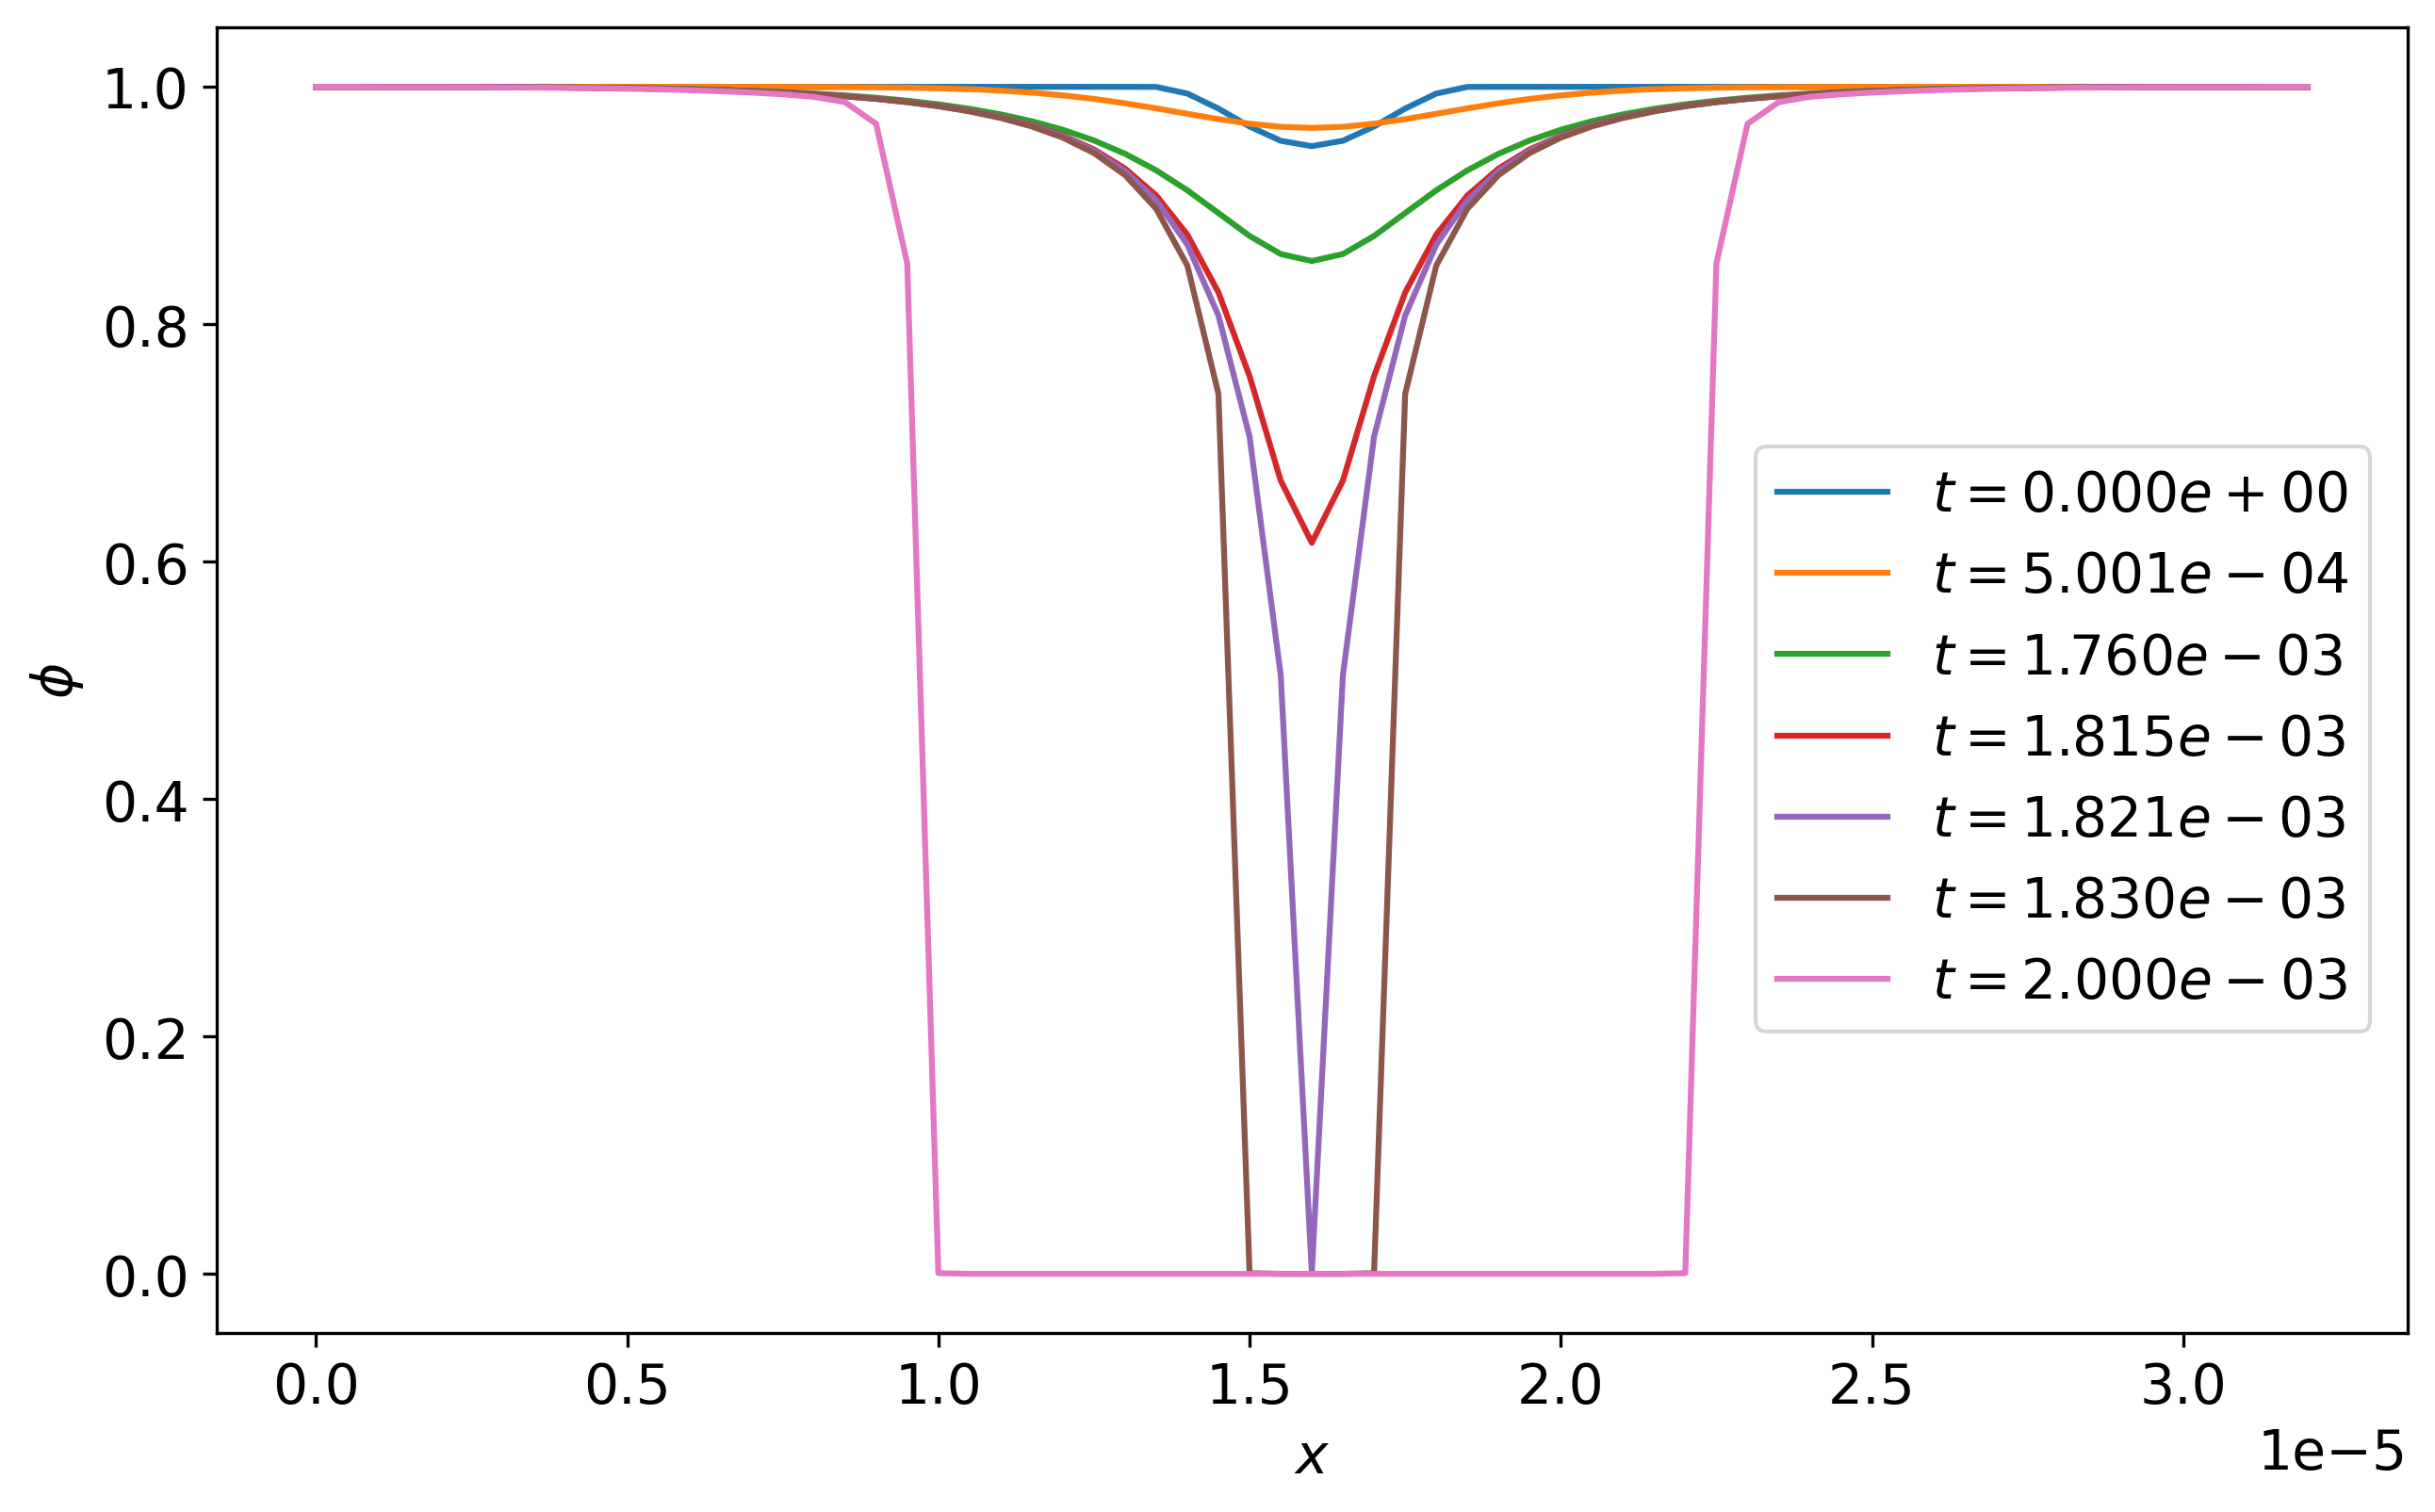
\includegraphics[width=0.81\textwidth]{figures/solution_basic.png}
\end{figure}
\end{frame}


\begin{frame}{Вычислительный эксперимент}
\vspace{-0.2cm}
\begin{center}
	Ошибка решения при ускорении
\end{center}
\vspace{-0.3cm}
\begin{figure}
	\hspace*{-0.5cm}
	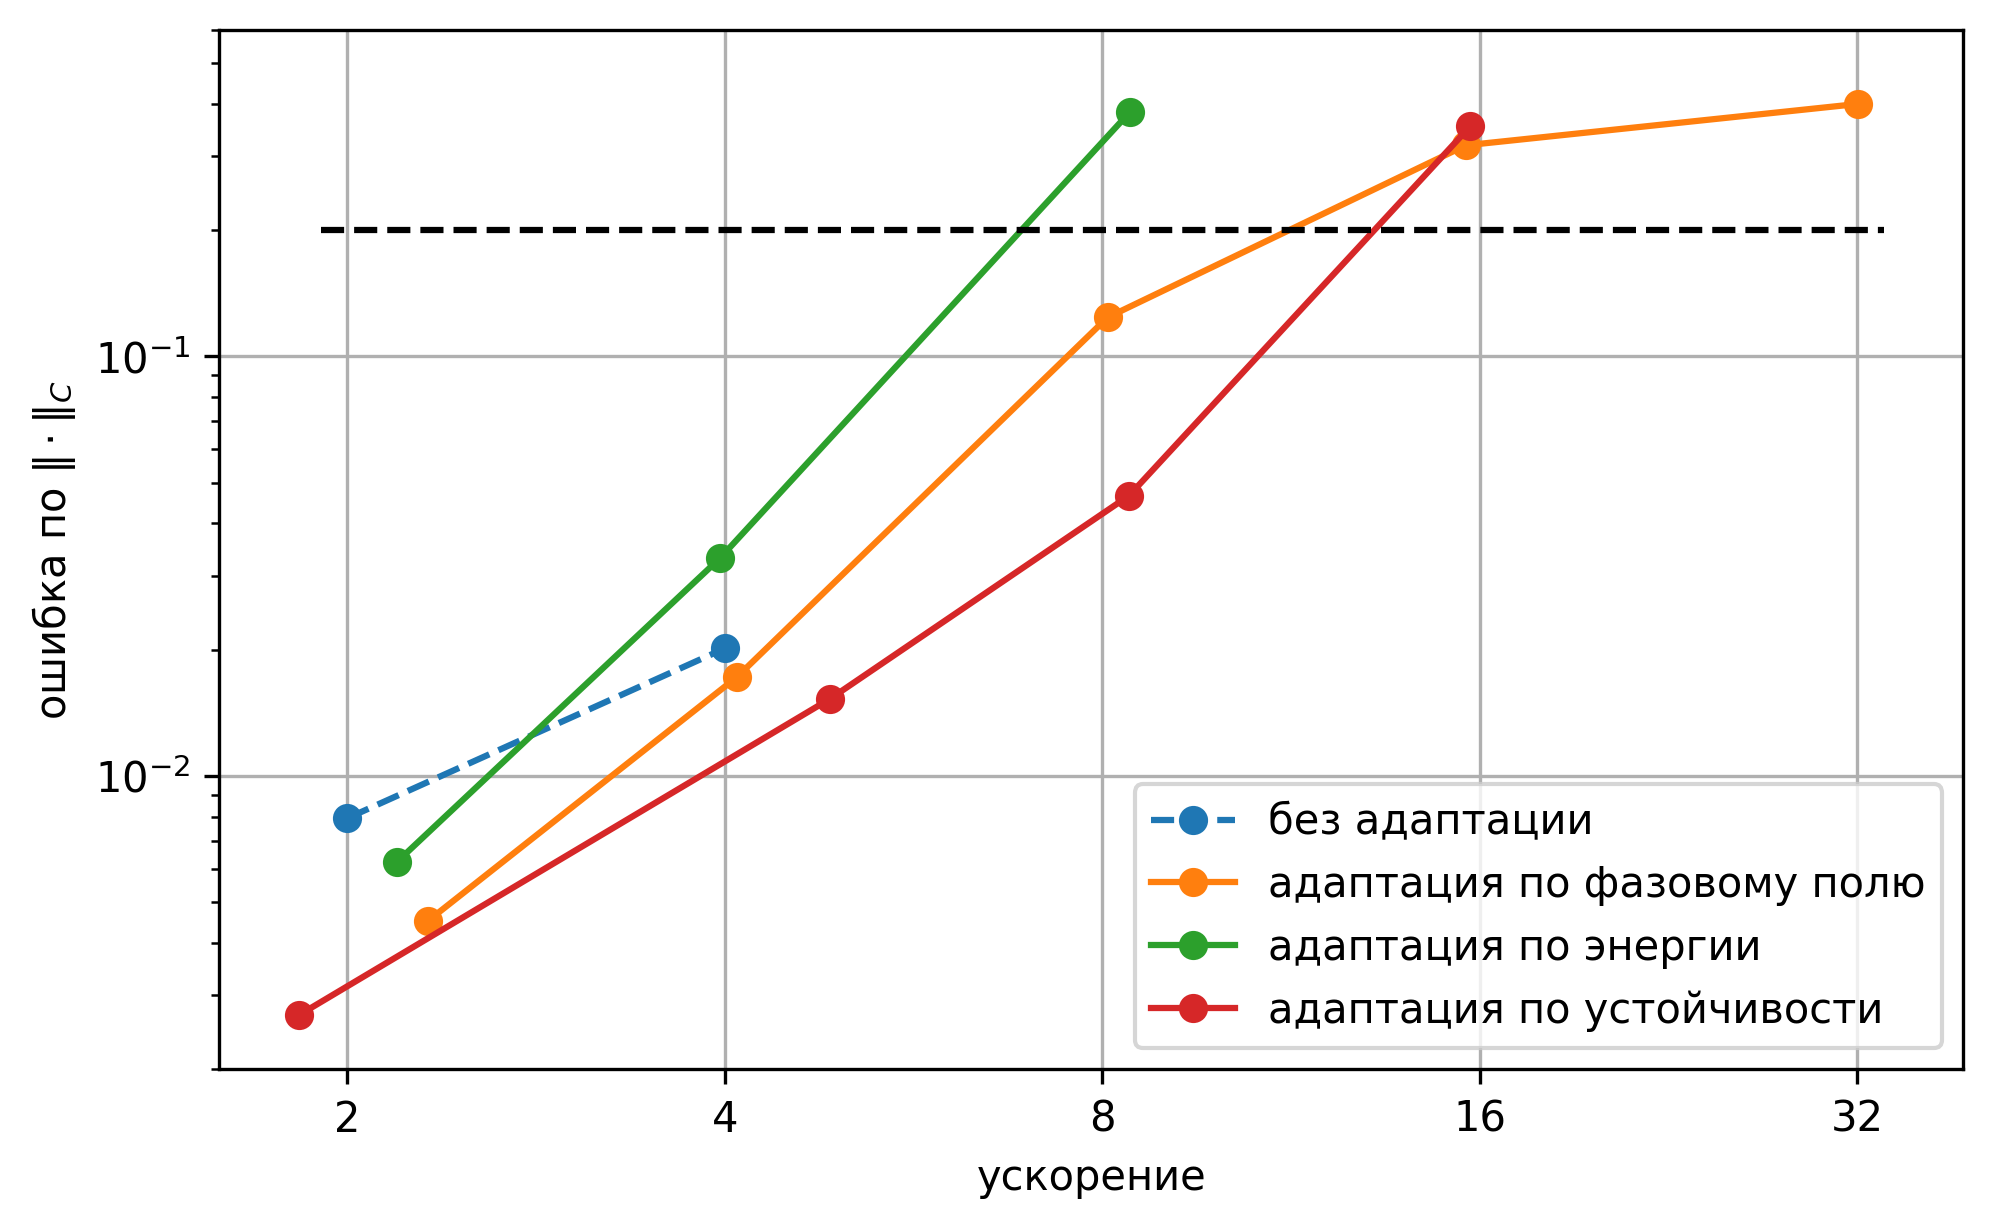
\includegraphics[width=0.75\textwidth]{figures/method_errors.png}
\end{figure}
\end{frame}


\begin{frame}{Вычислительный эксперимент}
\vspace{-0.2cm}
\begin{center}
	Ошибка решения при ускорении: задан существенный $\tau_{\max}$
\end{center}
\vspace{-0.3cm}
\begin{figure}
	\hspace*{-0.5cm}
	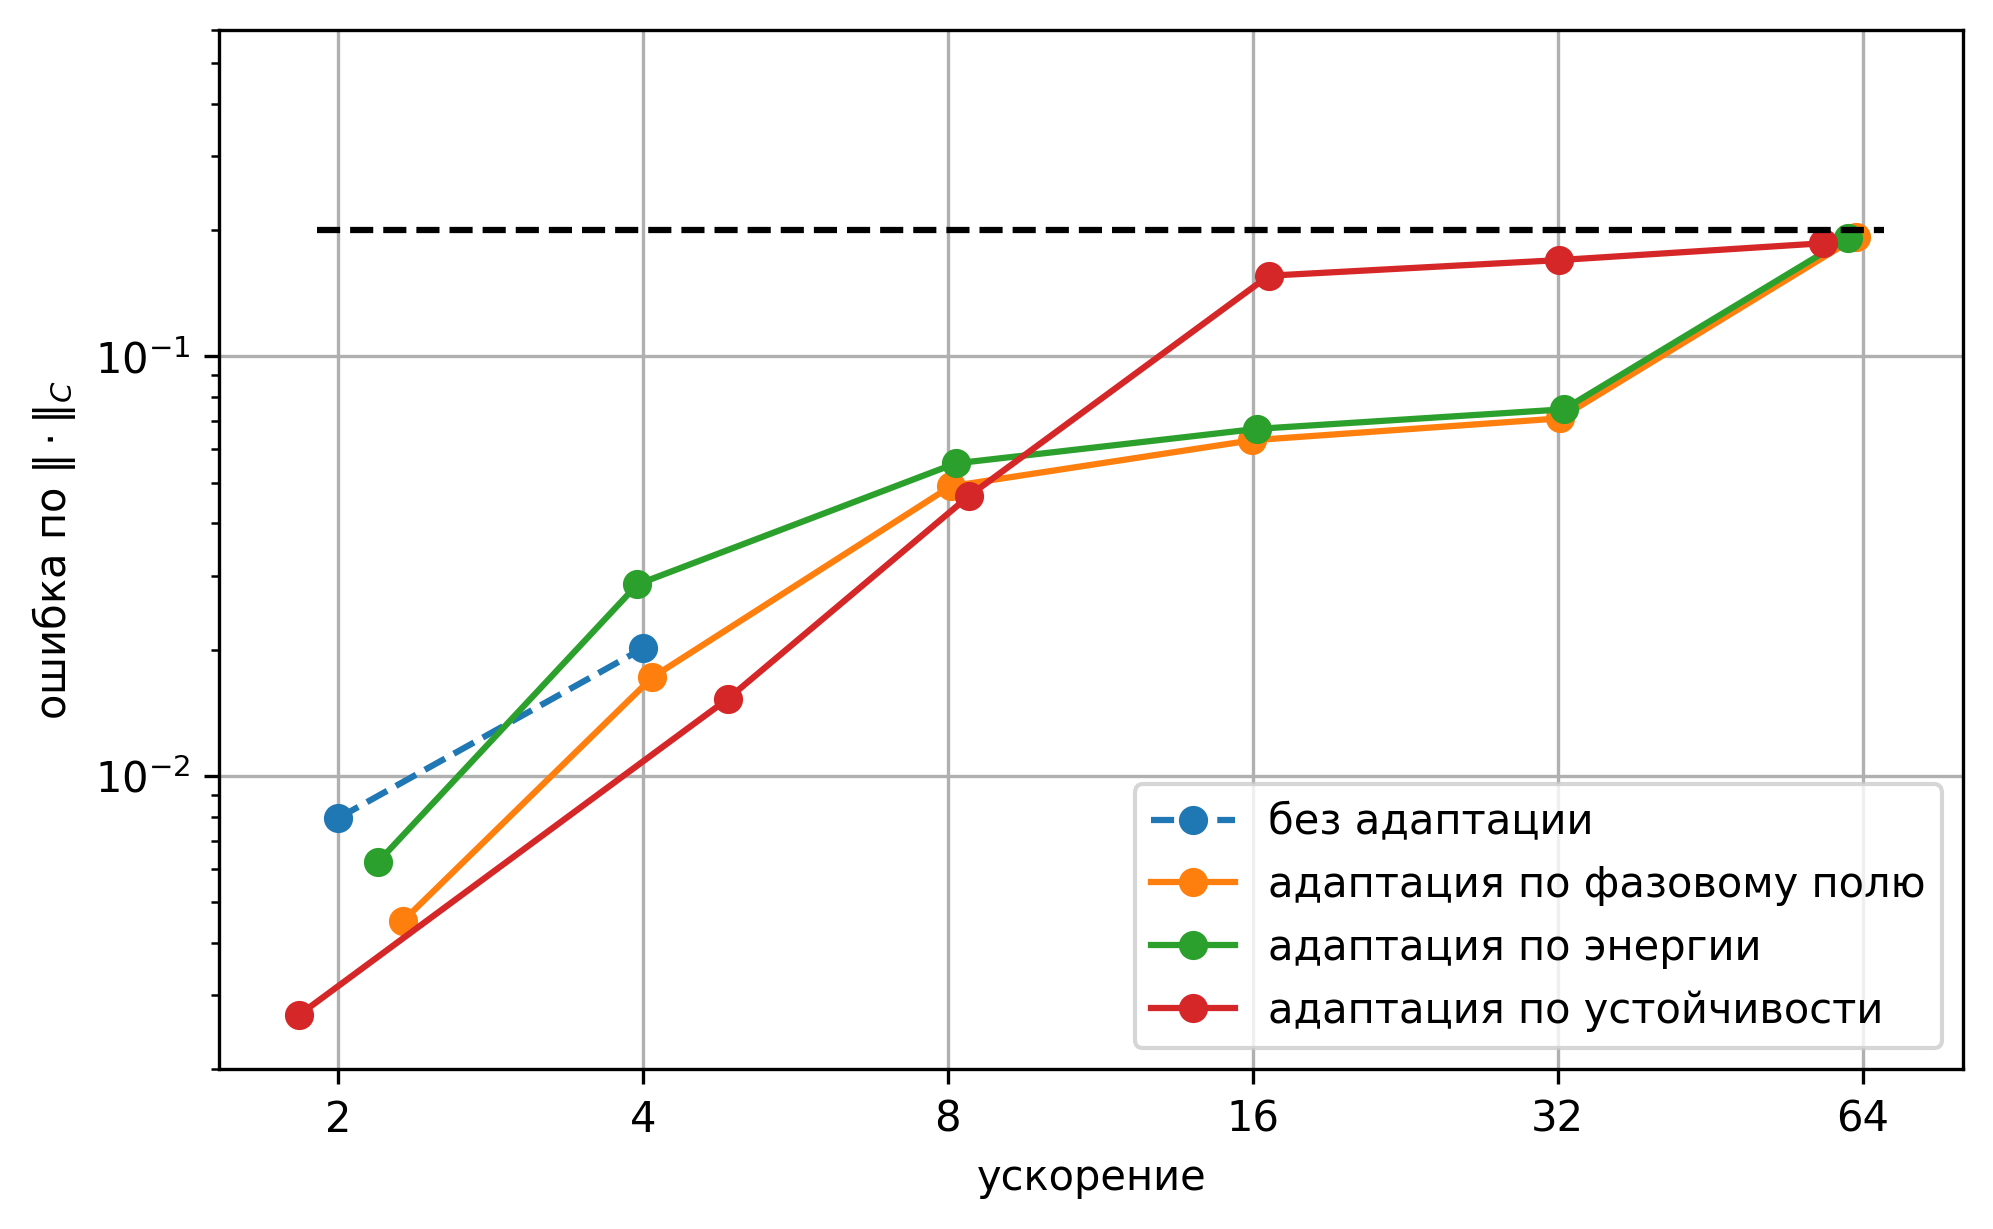
\includegraphics[width=0.75\textwidth]{figures/method_limited_errors.png}
\end{figure}
\end{frame}